\chapter{Symmetry, Invariance, and Conservation for Free Fields}
\section{Symmetry Mathematically}
The transformation depicted in Fig. (\ref{fig:cylinder-rot}) can be can be understood either as a rotation of the cylinder in one direction while we remain fixed (an \textbf{\underline{active transformation}}, by name), or alternatively, as a rotation of our viewing frame of reference in the other direction while the cylinder remains fixed (a\underline{ \textbf{passive transformation}}).
\begin{figure}[H]
    \centering
\tikzset{every picture/.style={line width=0.75pt}} %set default line width to 0.75pt        

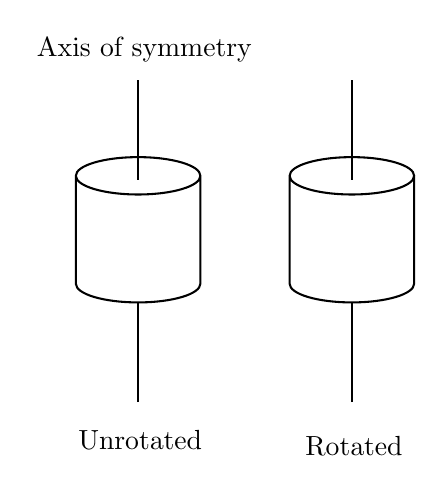
\begin{tikzpicture}[x=0.75pt,y=0.75pt,yscale=-1,xscale=1]
%uncomment if require: \path (0,300); %set diagram left start at 0, and has height of 300

%Shape: Can [id:dp6111663527038986] 
\draw   (154,122) -- (154,174) .. controls (154,178.97) and (140.57,183) .. (124,183) .. controls (107.43,183) and (94,178.97) .. (94,174) -- (94,122) .. controls (94,117.03) and (107.43,113) .. (124,113) .. controls (140.57,113) and (154,117.03) .. (154,122) .. controls (154,126.97) and (140.57,131) .. (124,131) .. controls (107.43,131) and (94,126.97) .. (94,122) ;
%Straight Lines [id:da6016989853853066] 
\draw    (124,124) -- (124,76) ;
%Straight Lines [id:da7742642520386162] 
\draw    (124,231) -- (124,183) ;
%Shape: Can [id:dp6333770541501842] 
\draw   (257,122) -- (257,174) .. controls (257,178.97) and (243.57,183) .. (227,183) .. controls (210.43,183) and (197,178.97) .. (197,174) -- (197,122) .. controls (197,117.03) and (210.43,113) .. (227,113) .. controls (243.57,113) and (257,117.03) .. (257,122) .. controls (257,126.97) and (243.57,131) .. (227,131) .. controls (210.43,131) and (197,126.97) .. (197,122) ;
%Straight Lines [id:da2230680788551479] 
\draw    (227,124) -- (227,76) ;
%Straight Lines [id:da2565843946616415] 
\draw    (227,231) -- (227,183) ;

% Text Node
\draw (125,249) node   [align=left] {Unrotated};
% Text Node
\draw (228,252) node   [align=left] {Rotated};
% Text Node
\draw (127,61) node   [align=left] {Axis of symmetry};


\end{tikzpicture}
    \caption{Symmetry of a cylinder}
    \label{fig:cylinder-rot}
\end{figure}
Mathematically, when we change our position of observation, it is equivalent to using a new, different reference frame and coordinate system, oriented differently from, and/or displaced relative to, the original. So a transformation can be viewed simply as a change of coordinate system, and this is often represented as a shifting from unprimed to primed coordinates. In QFT, \textbf{we will focus on passive transformation interpretation.}

\begin{example}
Consider the function 
\begin{equation}
g\left(x^{1}, x^{2}\right)=\left(x^{2}\right)^{2}
\end{equation}
if we have the following rorational transformation as
$$
\left[\begin{array}{l}
{x^{\prime 1}} \\
{x^{\prime 2}}
\end{array}\right]=\underbrace{\left[\begin{array}{cc}
{\cos \theta} & {\sin \theta} \\
{-\sin \theta} & {\cos \theta}
\end{array}\right]}_T\left[\begin{array}{l}
{x^{1}} \\
{x^{2}}
\end{array}\right]
\quad
\left[\begin{array}{l}
{x^{1}} \\
{x^{2}}
\end{array}\right]=\underbrace{\left[\begin{array}{ll}
{\cos \theta} & {-\sin \theta} \\
{\sin \theta} & {\cos \theta}
\end{array}\right]}_{T^{-1}=T^T}\left[\begin{array}{l}
{x^{\prime1}} \\
{x^{\prime2}}
\end{array}\right]
$$
we can express the function in the primed coordinate as:
$$
g=\left(x^{2}\right)^{2}=\left(x^{\prime 1} \sin \theta+x^{\prime 2} \cos \theta\right)^{2}=\left(x^{\prime 1}\right)^{2} \sin ^{2} \theta+\left(x^{\prime 2}\right)^{2} \cos ^{2} \theta+2 x^{\prime 1} x^{\prime 2} \sin \theta \cos \theta \neq\left(x^{\prime 2}\right)^{2}
$$
The transformed form of $g,$ represented by $g^{\prime}$, has the same value at the same physical point, but it is not the same form in terms of the primed coordinates as $g$ was in terms of the unprimed coordinates. But $f^{\prime},$ the transformed form of $f,$ did have the same form in terms of both sets of coordinates, and thus, we dropped the prime on $f$ on the RHS.

In spite of its non-symmetry under rotation, $g$ is symmetric under a different kind of Fransfort of the firc-symment ander founding $f$ the bynaced relative to the first along transformation, the translation to a coordinate system which is displaced relative to the first along the $x^{1}$ axis, i.e., $x^{1} \rightarrow x^{1}=x^{1}+$ constant $,$ or
$$
\left[\begin{array}{l}
{x^{\prime 1}} \\
{x^{\prime 2}}
\end{array}\right]=\left[\begin{array}{l}
{x^{1}} \\
{x^{2}}
\end{array}\right]+\left[\begin{array}{l}
{K} \\
{0}
\end{array}\right] \quad K=\text { constant }
$$
Substitution yields $g^{\prime}$ have the same form.
\end{example}
\begin{qt}
    From the example above, we can deduce the general rule that if a coordinate is missing in a given function, that function is invariant under a transformation solely in the direction of that coordinate (and also under multiplication of the coordiante by a constant).
\end{qt}
\textbf{\redp{So under any transformation of coordinate axes, the value at a physical point of every possible scalar function is invariant.}}
\subsection{Scalar are invariant, vectors are covariant}
\textbf{The scalar value at the point ( equal to the length of the position vector at that point) is the same in both systems, but the coordinate values are not.} For a 2D position vector in physical space, we have
$$
|x|=\left|x^{i}\right|=\sqrt{\left(x^{1}\right)^{2}+\left(x^{2}\right)^{2}}=\sqrt{\left(x^{\prime1}\right)^{2}+\left(x^{\prime2}\right)^{2}}=\left|x^{\prime i}\right|
$$
It is generally true of every vector $\mathbf{v},$ not just the position vector shown here, that its physical, measurable length (a scalar value) remains unchanged under any coordinate transformation, but its component values change. This is called covariance. Scalar values are invariant under coordinate transformation; vector components are \textbf{covariant}.
\begin{qt}
    General rule: if a function $h$ is not a function of the $j$th coordinate $x^j$, then h is symmetric under the transformation $x^{j} \rightarrow x^{j}+$ constant.
\end{qt}
\section{Symmetry in Classical Mechanics}
Recall that a Galilean transformation is
$$
\left[\begin{array}{c}
{x^{1}} \\
{x^{2}} \\
{x^{3}}
\end{array}\right] \rightarrow\left[\begin{array}{c}
{x^{11}} \\
{x^{\prime 2}} \\
{x^{3}}
\end{array}\right]=\left[\begin{array}{c}
{x^{1}-v^{1} t} \\
{x^{2}-v^{2} t} \\
{x^{3}-v^{3} t}
\end{array}\right]
$$
Newtonian mechanics is invariant under the Galilean transformation. But \textbf{Maxwell's eqs are not invariant under Galilean transformation. Instead, it is invariant under Lorentz transformation}
\begin{qt}
    \begin{equation}
\left[\begin{array}{c}
{x^{0}} \\
{x^{1}} \\
{x^{2}} \\
{x^{3}}
\end{array}\right] \rightarrow\left[\begin{array}{c}
{x^{\prime 0}} \\
{x^{\prime 1}} \\
{x^{\prime 2}} \\
{x^{\prime 3}}
\end{array}\right]=\left[\begin{array}{c}
{\gamma\left(x^{0}-\frac{v}{c} x^{1}\right)} \\
{\gamma\left(x^{1}-\frac{v}{c} x^{0}\right)} \\
{x^{2}} \\
{x^{3}}
\end{array}\right]=\underbrace{\left[\begin{array}{cccc}
{\gamma} & {-\gamma \frac{v}{c}} & {0} & {0} \\
{-\gamma \frac{v}{c}} & {\gamma} & {0} & {0} \\
{0} & {0} & {1} & {0} \\
{0} & {0} & {0} & {1}
\end{array}\right]}_{\Lambda}\left[\begin{array}{c}
{x^{0}} \\
{x^{1}} \\
{x^{2}} \\
{x^{3}}
\end{array}\right]
\label{lorentz-trans}
\end{equation}
where
$$
\gamma=\frac{1}{\sqrt{1-\frac{v^{2}}{c^{2}}}} \quad v=v^{1}
$$
\end{qt}
The index notation for Lorentz transformations is 
\begin{qt}
    \begin{equation}
x^{\prime \mu}=\Lambda^{\mu}{}_{v} x^{v} \quad V^{\prime \mu}\left(x^{\prime \alpha}\right)=\Lambda^{\mu}{}_{v} V^{v}\left(x^{\alpha}\right) \quad T^{\prime \mu v}\left(x^{\prime \alpha}\right)=\Lambda^{\mu}{}_{\delta} \Lambda^{v}{}_{\gamma} T^{\delta \gamma}\left(x^{\alpha}\right)
\end{equation}
Note that $\Lambda^{-1},$ the inverse of $\Lambda,$ can be obtained by taking $\mathbf{v} \rightarrow-\mathbf{v}$ since each coordinate system seems to be going in the opposite direction with respect to the other. $\Lambda^{-1}$ will transform $x^{\prime \mu}$ back into $x^{\mu}$.
\end{qt}
\bluep{Recall that the length of a vector in 3D is unchanged under a coordinate system transformation, 1.e., the length 1s a scalar and thus invariant. The same thing is true in 4D for four-vectors.}
$$
w_{\mu} w^{\mu}=w_{0} w^{0}+w_{1} w^{1}+w_{2} w^{2}+w_{3} w^{3}=w^{0} w^{0}-w^{1} w^{1}-w^{2} w^{2}-w^{3} w^{3}=\text { scalar invariant }
$$
\textbf{and that this is the same for any observer in any inertial coordinate system. This applies to any
vector, be it a position vector like $x^{\mu},$ the differential of position $d x^{\mu},$ the four-velocity $u^{\mu}$, the four potential $A^{\mu}$, the partial derivative $\partial^{\mu}$, or any other}.For instance,
$$
\frac{\partial}{\partial x^{\mu}} \frac{\partial}{\partial x_{\mu}}=\partial_{\mu} \partial^{\mu}=\frac{\partial}{\partial x^{0}} \frac{\partial}{\partial x^{0}}-\frac{\partial}{\partial x^{1}} \frac{\partial}{\partial x^{1}}-\frac{\partial}{\partial x^{2}} \frac{\partial}{\partial x^{2}}-\frac{\partial}{\partial x^{3}} \frac{\partial}{\partial x^{3}}=\text { scalar invariant derivative, }
$$
So if X represents a quantity, we have
$$
\frac{\partial}{\partial x^{\mu}} \frac{\partial}{\partial x_{\mu}}=\frac{\partial}{\partial x^{\prime \mu}} \frac{\partial}{\partial x_{\mu}^{\prime}} \rightarrow \frac{\partial}{\partial x^{\mu}} \frac{\partial}{\partial x_{\mu}} X=\frac{\partial}{\partial x^{\prime\mu}} \frac{\partial}{\partial x_{\mu}^{\prime}} X
$$
\subsection{Poincare transformation}
The most general transformation we could have in spacetime would comprise 1) a 4D translation(translating our coordinate axes in space, time, or both), 2) a rotation in space, and 3) a Lorentz transformation to a frame with different relative velocity. (We ignore reflection.)

The rotation in 3D is the same. It does allow us to rotate our 3D axes, however, so that the relative velocity between our original and transformed systems is along the $x^1$ axes of both. \textbf{This lets us use the Lorentz transformation in its simplest form (\ref{lorentz-trans})}. With this form we state the general transformation between coordinate systems, know as \redp{\textbf{Poincare transformation}} as
\begin{equation}
x^{\mu}=\Lambda_{\nu}^{\mu}\left(x^{\nu}+a^{\nu}\right) \quad a^{\nu}=\mathrm{constant} \text { four vector }
\label{poincare-trans}
\end{equation}

\subsection{Other kinds of symmetry}
Consider the Euler-Lagrange equation for a particle in Newtonian mechanics
$$
\frac{d}{d t}\left(\frac{\partial L}{\partial \dot{x}^{i}}\right)-\frac{\partial L}{\partial x^{i}}=0 \quad L=T-V \quad p_{i}=\frac{\partial L}{\partial \dot{x}^{i}}
$$
If the Lagrangian $L$ is not an explicit function of the spatial coordinate $x^i,$ then $\partial L / \partial x^{i}=0$ on the LHS above. Thus, the time derivative of $p_{i}$ is zero.
$$
\frac{d}{d t}\left(\frac{\partial L}{\partial \dot{x}^{i}}\right)=\frac{d p_{i}}{d t}=0 \quad \text { with } \frac{\partial L}{\partial x^{i}}=0 \quad \text { when } \quad L \neq L\left(x^{i}\right)
$$
Hence $p^i$ is constant and thus, conserved. This makes sense since the only source for spatial dependence in $L$ is the potential energy $V$. If we have no $V$ dependence on $x^i$, then there is no force in the $x^i$ direction, and momentum $p_i$ is constant.\textbf{Note this means the Lagrangian is symmtric.}

\redp{If the Lagrangian is symmetric in a coordinate, then the conjugate momentum for that coordiante is conserved.}